\documentclass[11pt,a4paper,openany,oneside]{book}
\usepackage[utf8]{inputenc}
\usepackage[french]{babel}
\bibliographystyle{unsrt}
\usepackage{graphicx}
\usepackage{ulem}
\usepackage[cyr]{aeguill}
\usepackage{hyperref}
\usepackage{natbib}
\usepackage[titletoc]{appendix}
\usepackage[acronym, xindy, toc, nonumberlist]{glossaries}
\usepackage{float}
\usepackage{listings}
\usepackage{color}
\usepackage{array}
\usepackage{lscape}
\usepackage{amsthm}
\usepackage{thmtools}

\addtolength{\topmargin}{-30pt}
\addtolength{\evensidemargin}{-50pt}
\addtolength{\oddsidemargin}{-50pt}
\addtolength{\textwidth}{100pt}
\addtolength{\textheight}{50pt}
\addtolength{\footskip}{12pt}
\renewcommand{\headsep}{25pt} 
\usepackage[utf8]{inputenc}

\definecolor{dkgreen}{rgb}{0,0.6,0}
\definecolor{gray}{rgb}{0.5,0.5,0.5}
\definecolor{mauve}{rgb}{0.58,0,0.82}

\renewcommand\thechapter {\Roman{chapter}}
\addto\captionsfrench{\renewcommand{\glossaryname}{Glossaire}}
\addto\captionsfrench{\renewcommand{\acronymname}{Acronymes}}
\setcounter{secnumdepth}{2}
\setcounter{tocdepth}{2}

\lstset{frame=tb,
  defaultdialect=Java,
  aboveskip=3mm,
  belowskip=3mm,
  showstringspaces=false,
  columns=flexible,
  basicstyle={\small\ttfamily},
  numbers=none,
  numberstyle=\tiny\color{gray},
  keywordstyle=\color{blue},
  commentstyle=\color{dkgreen},
  stringstyle=\color{mauve},
  breaklines=true,
  breakatwhitespace=true,
  numbers=left,
  frame = single,
  tabsize=3
}

\definecolor{dkgreen2}{rgb}{0.1,0.8,0.1}
\definecolor{gray2}{rgb}{0.7,0.3,0.2}
\definecolor{mauve2}{rgb}{0.5,0.5,0.8}


\lstdefinelanguage{Compo}
{keywords={
connect, delegate, to, architecture, service, provides, requires, internally requires, extends, Descriptor, provides, service, internally, rockonnect, disconnect, operation, return},
sensitive=true,
alsoletter={\$},
comment=[l]{\#},
string=[b]",
morecomment=[s]{"}{"},
string=[b]'
}



\lstset{frame=tb,
  defaultdialect=Compo,
  aboveskip=3mm,
  belowskip=3mm,
  showstringspaces=false,
  columns=flexible,
  basicstyle={\small\ttfamily},
  numbers=none,
  numberstyle=\tiny\color{gray},
  keywordstyle=\color{blue},
  commentstyle=\color{dkgreen},
  stringstyle=\color{mauve},
  breaklines=true,
  breakatwhitespace=true,
  numbers=left,
  frame = single,
  tabsize=3
}



\title{Analyse d'un langage de programmation réflexif orienté composants \\ Etude de COMPO}

\author{Anthony Ferrand \and Lucas Nelaupe \and Frédéric Verdier}

\date\today

\begin{document}

\maketitle

\chapter*{Remerciements}

Nous souhaitons remercier avant tout Monsieur Dony, notre tuteur lors du projet, pour ses très nombreux conseils et son regard critique et exigeant sur notre travail.\\
Nous remercions aussi Monsieur Petr Spacek, créateur du langage COMPO, qui a bien voulu nous aider en répondant à toutes nos questions. \\
Nous remercions également Monsieur Tibermacine, chercheur au LIRMM, pour ses nombreuses idées et interventions dans le cadre de notre projet.\\



\tableofcontents

\chapter{Introduction}

\section{Définitions}

\subsubsection{Composant}

\textit{"A run-time entity which provides and requires services through ports"} [Définition de composant dans \citep{these}].\\
Un composant est un élément du programme. Celui-ci sera couplé à d'autres pour former un programme.
\subsubsection{Port}

\textit{"Un port est un point de connexion (les composants sont connectés par leurs ports) et de communication (les invocations de services sont transmises via les ports)."} [Définition de port dans \citep{articleToRead}].\\
Les composants peuvent communiquer entre eux grâce à des envois de messages via leurs ports.

\subsubsection{Connexion}

\textit{"Describes a binding from one to another port"} [Définition de connexion dans \citep{these}].\\
Une connexion représente un lien ou une voie de communication entre deux ports. C'est par ce biais que seront effectué les envois de messages.

\section{Contexte : La réutilisabilité en développement logiciel}

Développer un logiciel est très coûteux. Cependant, certains éléments sont redondants entre tous les logiciels. Le but est de ne concevoir qu'une seule fois ce dont on a besoin. Si un programme a besoin d'un service que l'on a déjà développé pour un précédent logiciel, l'architecte n'aura qu'à reprendre le précédent service déjà développé qui fournit ce dont il a besoin. On peut également imaginer une banque de composants considérés comme fiables par la profession. Cette banque serait disponible via Internet. Cela comporte un double avantage. D'une part, le développement logiciel sera d'autant plus rapide et donc moins coûteux. D'autre part, vu que ces composants sont déjà testés, le programme sera moins sujet aux erreurs.

\subsection{Comment développer un programme pour que ses éléments soit réutilisables?}

Les différents paradigmes de programmation majoritairement utilisés dans les langages ne permettent pas ou très peu la réutilisation. Actuellement, la réutilisabilité se limite surtout aux bibliothèques de logiciels qui ont été faites pour être réutilisables.

\subsection{Solution : La programmation orientée composants}

Il existe un paradigme de programmation qui facilite la réutilisation : le paradigme composant. Chaque partie du programme est cloisonnée et a des tâches précises. Le tout fonctionne par des envois de messages. Cette séparation permet donc facilement de récupérer une partie du programme qui nous servira pour un autre.

\section{Objectifs : Comprendre et améliorer le langage COMPO}

Il existe actuellement, très peu de langages  permettant de faire de la programmation par composants qui spécifient la logique métier d'un programme. En effet la majorité des langages de programmation de ce type sont des ADL (\textit{Architecture Description Language}). Ils ne décrivent que l'architecture générale d'un programme et utilisent des exécutables écrits dans d'autres langages pour la logique métier (Java, C++, ...).\\ 
Nous avons cependant trouvé le langage COMPO, actuellement à l'état de prototype, et avons décidé de participer à son développement.

\chapter{Le langage COMPO}

COMPO est un langage réflexif de programmation et de modélisation orienté composants. Ce chapitre propose une approche pour se familiariser avec le langage.\\
Nous utiliserons les termes présents dans la version actuelle de COMPO.

\section{Les descripteurs de composants}

Les composants sont décrits par un descripteur. Un composant est une instance du descripteur le décrivant. On peut faire le parallèle avec la programmation orientée objets où les objets sont des instances de classes.\\
Les descripteurs sont eux-mêmes des composants décrits par leur méta-descripteur (\texttt{Descriptor} par défaut).

\begin{figure}[H]
	\centering
	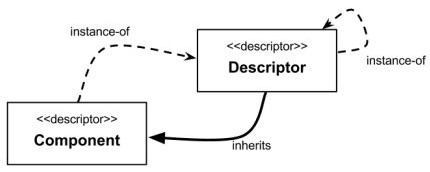
\includegraphics[keepaspectratio = true]{metamodel}
	\caption{Métamodèle du langage COMPO extrait de \citep{these}}
	\label{MetaModel}
\end{figure}

\subsection{Les informations présentes dans un descripteur}

Afin de décrire un composant, il est nécessaire d'expliciter :
\begin{description}
\item[Le requis]Ce dont un composant a besoin pour fonctionner. Ici ces requis pourront être fournis grâce à d'autres composants.
\item[Le fourni]Il s'agit des services que le composant décrit propose. Ces services pourront ainsi être proposés à d'autres composants.
\item[Les services]COMPO étant un langage décrivant aussi la logique métier des composants. Cette logique métier se trouve dans les services des composants. Donc le descripteur doit aussi décrire le contenu des services proposés.
\item[Les connexions entre composants internes]Les composants peuvent être eux-mêmes composés d'autres composants. On parle alors de \textbf{composites}. L'utilisateur d'un composite ne connaîtra pas ses connexions internes. C'est pourquoi le développeur ayant créé le descripteur doit pouvoir spécifier les connexions internes.
\end{description}


\subsection{Instanciation d'un composant}

Pour créer une nouvelle instance d'un descripteur, il faut utiliser le service \texttt{new()}.\\
Ce service est présent dans tous les composants et renvoie le port fourni par défaut \texttt{default} d'une nouvelle instance du descripteur receveur courant.\\
Voici la syntaxe d'utilisation de \texttt{new()} : 
\begin{lstlisting}[language=Compo, frame=single, caption=Syntaxe de création d'un nouveau composant]
<Descripteur>.new();
\end{lstlisting}

\subsection{Exemple de syntaxe d'un descripteur en COMPO}

Maintenant que nous avons introduit les concepts de ports, services et descripteurs, nous allons donner la syntaxe générale d'un descripteur.
\begin{lstlisting}[language=Compo, frame=single, caption=Syntaxe générale d'un descripteur]
<Meta-descripteur> <Descripteur> extends <Super-descripteur>{
    provides {
        //ports fournis
        <Declaration de port>
    }
    requires {
        //ports requis
        <Declaration de port>
    }
    internally requires {
        //ports internes requis
        <Declaration de port>
    }
    architecture {
        //Connexions interne
        <instructions de connexion>
    }
    //Definition des services
    <Services>
}
\end{lstlisting}

\clearpage

\section{Les ports}

Un composant peut communiquer avec d'autres composants via ses ports. Un port est défini par un nom, une liste de signature de services proposée, une visibilité, un rôle et une cardinalité.

\subsection{Rôle}

Un port peut avoir deux rôles : fournis (\texttt{provides}) ou requis (\texttt{requires}).

\subsubsection{Fournis}

Un port fournit, liste les signatures de services qui sont offerts par un composant. 

\subsubsection{Requis}

Un port requis; liste les signatures de services que le composant requiert pour fonctionner.

\subsection{Visibilité}

Un port peut être soit interne, soit externe.\\
Un port interne ne sera pas visible (accessible) depuis l'environnement extérieur du composant. Ces ports servent à réaliser les connexions entre un composite et ses composants internes.\\
Un port externe est visible depuis l'environnement extérieur du composant. Il peut être connecté à un autre composant.\\
Par défaut un port est externe. Il faut préciser sa visibilité interne (\texttt{internally}) lorsqu'on veut un port interne.

\subsection{Cardinalité}

Un port peut être simple ou multiple.\\
Un port simple peut être connecté à un autre port tandis qu'un port multiple est une collection de ports simples. Chacun des ports doit avoir la même liste de signatures de services.

\subsection{Les ports par défaut}

Tous les composants possèdent un port fourni externe par défaut nommé \textbf{default} qui fourni tous les services publiques du composant.\\
Ils ont aussi un port interne requis unique nommé \textbf{self} listant l'ensemble des services qu'ils possèdent.\\
Les composants possèdent également un autre port requis interne nommé \texttt{super}, connecté au composant descripteur parent.\\
Enfin ils possèdent un port externe requis multiple nommé \texttt{args}. Ce port permet lors d'une invocation de service de stocker les arguments s'il y en a.


\begin{figure}[H]
\centering
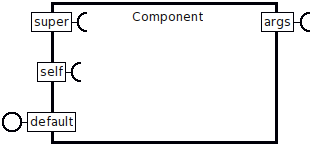
\includegraphics[scale=0.7, keepaspectratio=true]{compo}
\caption{Schéma d'un composant avec ses ports par défauts}
\label{args}
\end{figure}

\subsection{Syntaxe générale de définition d'un port}

Voici la syntaxe d'une clause de ports : \\
\begin{lstlisting}[frame=single,caption=Syntaxe de la déclaration d'un port]
<visibilite> <role> {
    //Definition de la liste des services par extension
    <Nom de port>:{ <signature service>; ... };
    //ou par interface/descripteur
    <Nom de port multiple>[]:<Interface||descripteur>;
    ...
}
\end{lstlisting}

\section{Les connexions}

Les connexions permettent de lier des ports entre eux et ainsi de transmettre des invocations de service entre ports connectés.
Les connexions dans COMPO peuvent être de deux types : connexion standard ou délégation.

\subsection{Standard : requis-fourni}

Une connexion classique permet de connecter un port requis avec un port fourni. Le port fourni ne peut être connecté à un port requis que si l'ensemble des signatures de services du port requis est un sous-ensemble de celui des signatures de services du port fourni.

\begin{lstlisting}[language=Compo, frame=single, caption=Syntaxe de la connexion]
//Connexion
connect <port>@<composant> to <port>@<composant>; 
\end{lstlisting}

\subsection{Délégation : requis-requis ou fourni-fourni}
Une délégation se fait entre deux ports de même rôle. Elle sert à déléguer l'invocation de service d'un port à l'autre. Cette délégation n'est possible que si l'ensemble des signatures de services du port délégant est au moins un sous-ensemble des signatures de services du port à qui on délégue les invocations.

\begin{lstlisting}[language=Compo, frame=single, caption=Syntaxe de la délégation]
//Delegation
delegate <port>@<composant> to <port>@<composant>;
\end{lstlisting}

\section{Architecture interne}

Un descripteur peut décrire l'architecture interne d'un composite grâce à la clause \texttt{architecture}.\\
Cette clause est une série d'instructions appelées à l'instanciation du composant permettant de créer sa structure interne. On y trouve ainsi l'ensemble des connexions à réaliser pour initialiser le composant dans ses ports internes.

La clause d'architecture interne se définit de la façon suivante. 

\begin{lstlisting}[language=Compo, caption=Syntaxe de la définition d'une clause architecture, frame=single]
architecture {
    <instructions de connexion>
}
\end{lstlisting}

\section{Les services}

Les services implémentent la logique métier (ou comportement) du composant. Ils peuvent prendre des paramètres et retourner un composant par un de ses ports fournis.

\subsection{L'invocation}

L'invocation de service se fait à partir d'un port requis connecté à un port fourni passé sous forme d'argument.
\begin{lstlisting}[frame=single, caption=Syntaxe de l'invocation de service]
<portRequis>.<service>(<param1>, <param2...>);
\end{lstlisting}

\subsection{Les arguments}

Tous les composants possèdent un port externe nommé \texttt{args}. Lors de l'invocation d'un service, les composants passés en paramètre sont automatiquement connectés à ce port. Lors de l'exécution du service, l'appelé va automatiquement récupérer le composant concerné au port \texttt{args}.

\subsection{Syntaxe générale d'un service}

Un service est défini dans un descripteur avec la syntaxe suivante : 
\begin{lstlisting}[language=Compo, frame=single, caption=Syntaxe de la définition d'un service]
service <Nom>(<Parametre>, ...) {
    <Instructions>
}
\end{lstlisting}

\chapter{Réflexion sur les améliorations possibles de COMPO}

\chaptermark{Améliorations possibles de COMPO}

\section{Analyse des connexions}

\subsection{Connexion standard}

Elle s'apparente aux passages d'arguments Java. A savoir : le composant passé en argument peut être modifié, mais la variable extérieure gardera un lien sur celle-ci. La variable dans l'appel de la fonction et la variable dans les arguments de la fonction ne sont pas liées. La modification de l'une ne changera pas l'autre. On passe donc une référence vers le composant. Ce comportement est semblable à celui de C++ lorsqu'on utilise un passage d'arguments par \&. L'affectation d'une variable de type T\& changera la valeur, et non le pointeur vers celle-ci.

\subsection{Délégation}
    		
Elle n'existe pas de façon non-programmatique en Java, mais son comportement peux être simulé par la création d'un objet intermédiaire. Idem pour C++. En effet, pour simuler cette connexion, il faudrait simuler un passage de pointeur \textit{immutable}, qui contiendrai une référence vers l'objet. Un exemple est donné en annexe \ref{Annexe A} avec une implémention en Java.

\subsection{Connexion partagée : \{requis\}-fourni}
\label{connexionPartageeRef}
Une connexion \{requis\}-fourni consiste à connecter un ensemble de ports requis à un port fourni.\\ 
Si un des ports requis modifie la connexion, alors les autres ports requis seront modifiés de la même manière.\\
Contrairement à la délégation, tous les ports peuvent modifier cette connexion. La figure~\ref{connexionPartagee} illustre l'idée proposée.
\begin{figure}[H]
\centering
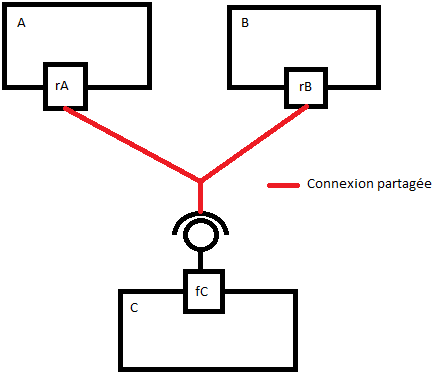
\includegraphics[scale=0.7, keepaspectratio=true]{connexionPartagee.png}
\caption{Schéma d'une connexion partagée}
\label{connexionPartagee}
\end{figure}

\subsubsection{Implémentation}
Il n'existe pas de solution simple directement implémentable en COMPO. Voici néanmoins des solutions possibles d'extension du langage.

\paragraph{Solution 1 : Passer par un composant gérant le partage}
Cette solution implique d'ajouter un composant intermédiaire pour partager une connexion entre plusieurs composants. Voir figure \ref{solution1}.
\begin{figure}[H]
\centering
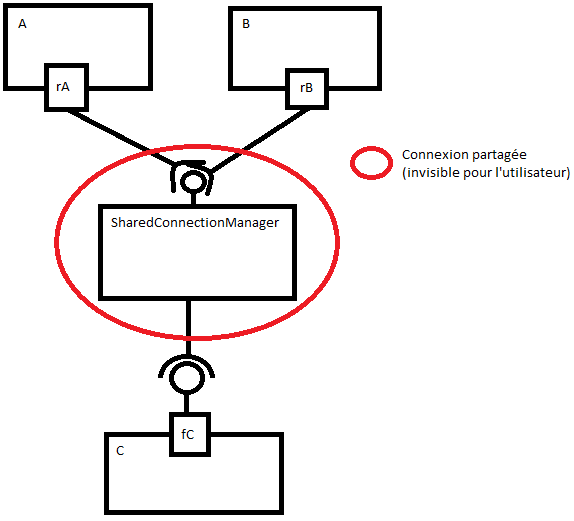
\includegraphics[scale=0.7, keepaspectratio=true]{solution1.png}R
\caption{Solution 1 : le composant \texttt{SharedConnectionManager} gère le partage de la connexion entre \texttt{A} et \texttt{B} vers \texttt{C}}
\label{solution1}
\end{figure}
Le composant intermédiaire offre des opérations de connexion, déconnexion de son port requis via son port fourni.\\
Les composants connectés au composant instance de \texttt{SharedConnectionManager} peuvent ainsi modifier par envois de messages la connexion entre le composant intermédiaire et \texttt{C} (impactant donc tous les autres composants).\\
Afin de rendre invisible ce composant intermédiaire, il est nécessaire de modifier les ports requis actuels. Un port requis posséderait un booléen \texttt{isSharing}, vrai si et seulement si le port est connecté à un composant de connexion partagée intermédiaire. De plus il faudrait modifier les opérations \texttt{connectTo} (pour se connecter à un port fourni) et \texttt{disconnect} (pour se déconnecter d'un port fourni) afin de ne pas couper sa connexion avec le composant intermédiaire mais au contraire faire appel à son opération correspondante (si \texttt{isSharing} est vrai). A cela devra être rajouté une opération \texttt{endSharedConnection} afin de rompre la connexion entre le port et l'instance de \texttt{SharedConnexionManager}.\\
Cette solution peut être actuellement implémentée dans COMPO sans modification du langage si on laisse le composant intermédiaire visible. Cela implique que le contenu des opérations des composants \texttt{A} et \texttt{B} doit prévoir une telle connexion partagée. C'est pourquoi il est préférable que la gestion de cette connexion partagée soit directement effectuée dans les ports.

\paragraph{Solution 2 : Créer un nouveau type de port requis}
Cette solution propose d'augmenter le langage COMPO avec un nouveau type de port évitant le passage par un composant intermédiaire. La figure~\ref{solution2} représente une implémentation de cette solution.\\
\begin{figure}[H]
\centering
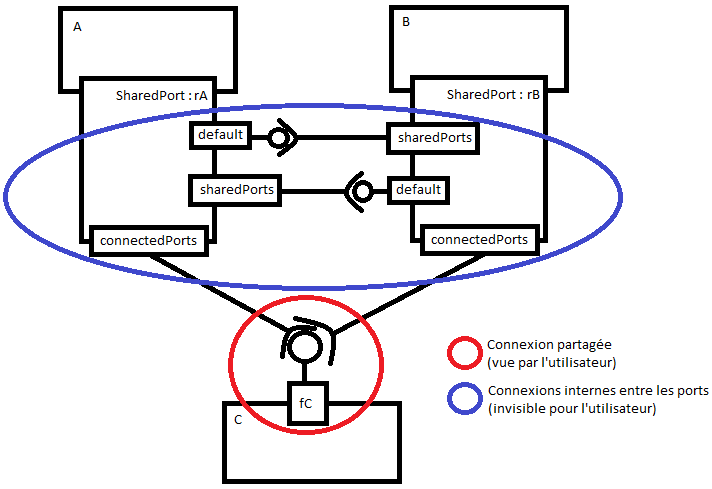
\includegraphics[scale=0.7, keepaspectratio=true]{solution2.png}
\caption{Solution 2 : on utilise un port de type \texttt{SharedPort} pour créer une connexion partagée}
\label{solution2}
\end{figure}
Ici on utilise un nouveau type de port nommé \texttt{SharedPort}. Celui-ci possède un port requis supplémentaire aux ports classiques \texttt{sharedPorts} qui sera connecté au port \texttt{default} d'un autre port instance de \texttt{SharedPort}.\\
Ce nouveau port devra redéfinir ses opérations \texttt{connectTo} et \texttt{disconnect} afin d'appeler l'opération correspondante via son port \texttt{sharedPorts}.\\
Grâce à l'utilisation d'une syntaxe adéquate, il est possible de rendre les connexions entre les ports qui partagent une connexion invisible pour l'utilisateur qui aura l'impression d'utiliser un port classique.

\paragraph{Solution préconisée}
La solution 2 demande 4 connexions pour chaque paire de connexion. Cela fait donc $2n$ connexions avec n le nombre de composants partagés.\\
La solution 1 demande une connexion pour chaque composant partagé plus une connexion entre le composant intermédiaire et la cible. On obtient donc $n+1$ connexions.\\
La solution 1 est donc plus économe en nombre de connexions dans tous les cas ($n>1$). Nous préconisons donc l'utilisation de la première solution.

\subsubsection{Cas d'utilisation}
Un composant ne peut pas anticiper comment il sera utilisé. Cela implique qu'un composant ne peut pas déterminer quel type de connexion sera utilisé sur ses ports requis externes.\\
Par conséquent, pour une connexion E-fourni où E est un ensemble de ports requis, tout composant ayant un port requis externe appartenant à E ne peut initialiser la connexion (car sinon il anticiperait son utilisation).

\subsubsection{Syntaxe proposée}
Contrairement à la connexion standard ou à la délégation, la connexion partagée ne peut être implémentée rapidement par un utilisateur du langage COMPO. Il faut donc l'autoriser avec un raccourci syntaxique qui mettra en place automatiquement l'une des solutions proposées.\\
Par exemple on peut imaginer la syntaxe suivante : 
\begin{lstlisting}[language=Compo, frame=single,caption=Syntaxe de création d'une connexion partagée]
connect {<portRequis>,<portRequis>} to <portFourni>;
\end{lstlisting}

\subsubsection{Comparaison avec C++}
		
La connexion partagée (voir figure~\ref{connexionPartagee}) ne possède pas d'équivalent en Java. Cependant en C/C++ elle s'apparente à l'utilisation de pointeurs. Ces pointeurs pointent sur la même adresse mémoire. Lorsque la valeur à cette adresse est modifiée, elle l'est pour toutes les variables pointant sur cette adresse. On retrouve ce comportement dans la connexion partagée où les ports requis sont des pointeurs pointant sur la même adresse mémoire (ici le port fourni).

\begin{lstlisting}[language=C++, frame=single, caption=Exemple en c++]
int *i = new int;
int *j = i;
*i = 5;
cout << *j << endl; // Affiche : 5
\end{lstlisting}

\subsection{Conclusion}
L'étude des autres langages a mis le doigt sur le fait que COMPO introduit une nouvelle façon de considérer le "passage de variables". Ce passage inédit est le passage par port requis (délégation). Bien que pouvant être simulé dans Java et C++.\\
De plus COMPO reprend les deux mécanismes principaux pour récupérer une valeur : par référence Java (connexion requis-fourni) ou par pointeur dé-référencé C++ (connexion \{requis\}-fourni).

\newpage

\section{Passage d'arguments}

COMPO est un langage dont la communication entre composants est représentée par l'invocation de service par leurs ports requis.\\
Un service est très similaire aux méthodes de classe dans un langage orienté objets.\\
Comme pour une méthode, un service peut prendre des arguments.
Actuellement, les arguments des services de COMPO sont des ports requis internes du receveur courant représentés par le port multiple \texttt{args}.\\
A l'invocation du service, on passe alors des ports fournis en arguments qui seront connectés à \texttt{args} avant l'exécution du corps. On obtient alors des connexions temporaires entre le receveur courant et les composants passés en argument.\\ 
Si on pouvait diversifier le type des paramètres proposés, il pourrait être intéressant de permettre à un même service d'avoir des comportements différents en fonction des types d'arguments proposés (surtout dans le cas où un service utilisera l'argument pour le connecter à un de ses ports).


\subsection{Par composant}
On peut dans un premier temps se demander si un argument représente un port ou un composant.\\
Dans la programmation orientée composants, on peut communiquer avec un composant que grâce à ses ports. Il ne sert donc à rien de passer en argument un composant directement, car on ne peut que passer par ses ports pour communiquer.\\
De manière générale, pour référencer une valeur, une "variable" devra toujours passer par un port du composant ciblé. Ainsi un argument ne peut avoir pour valeur qu'un port.

\clearpage

\subsection{Par port fourni}
\label{passageFourni}

Dans ce cas on passe en argument un port fourni (mode de passage d'arguments actuellement utilisé dans COMPO), on obtient une architecture représentée par la figure~\ref{exempleFourni}.\\
\begin{figure}[H]
\centering
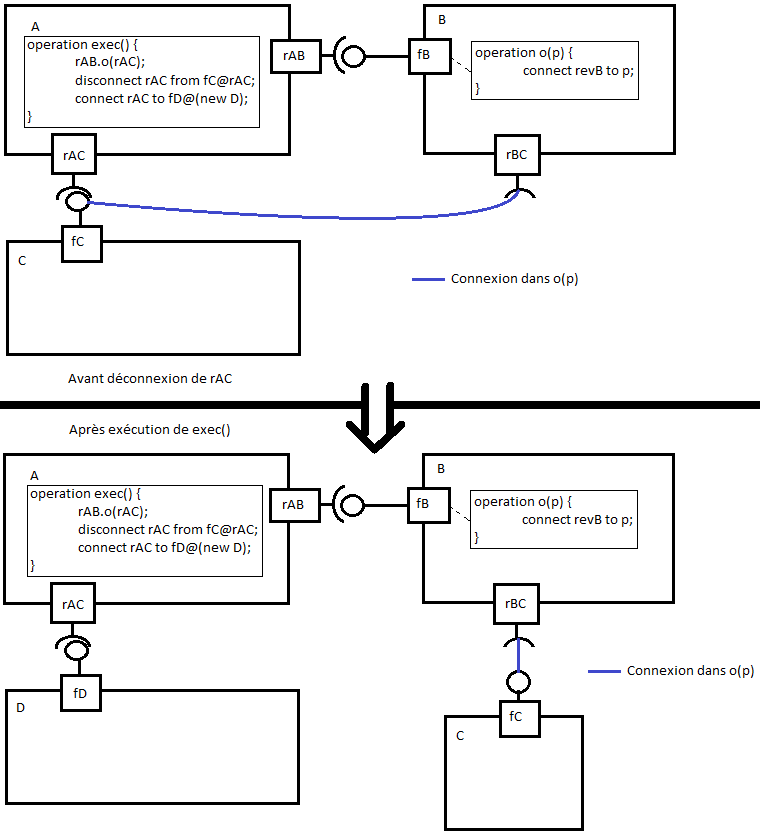
\includegraphics[scale=0.7, keepaspectratio=true]{exempleFourni.png}
\caption{Exemple lors d'un passage d'un port fourni en argument à \texttt{o}}
\label{exempleFourni}
\end{figure}
On remarque que la connexion entre \texttt{rBC} et \texttt{fC} est conservée après la connexion de \texttt{rAC} à \texttt{fD}.
Le passage d'un port fourni est comparable au passage d'arguments par références de Java.

\begin{lstlisting}[language=Java, caption=Equivalent en Java d'un passage de port fourni en paramètre de \texttt{o}]
public void o(Port p) {
    this.rBC = p;    
}
\end{lstlisting}


\subsection{Par port requis}

\label{passageRequis}
On suppose pouvoir passer en paramètre de \texttt{o} le port requis et non le port fourni auquel il est connecté. \\
On suppose également que l'instruction "\texttt{connect <portRequis> to <portRequis>;}" crée une délégation du premier port vers le second car sinon on ne pourrait pas exécuter \texttt{exec()} sans lever une exception.\\
La figure~\ref{exempleRequis} montre ce que l'on obtient lors de l'exécution de \texttt{exec()}.
\begin{figure}[H]
\centering
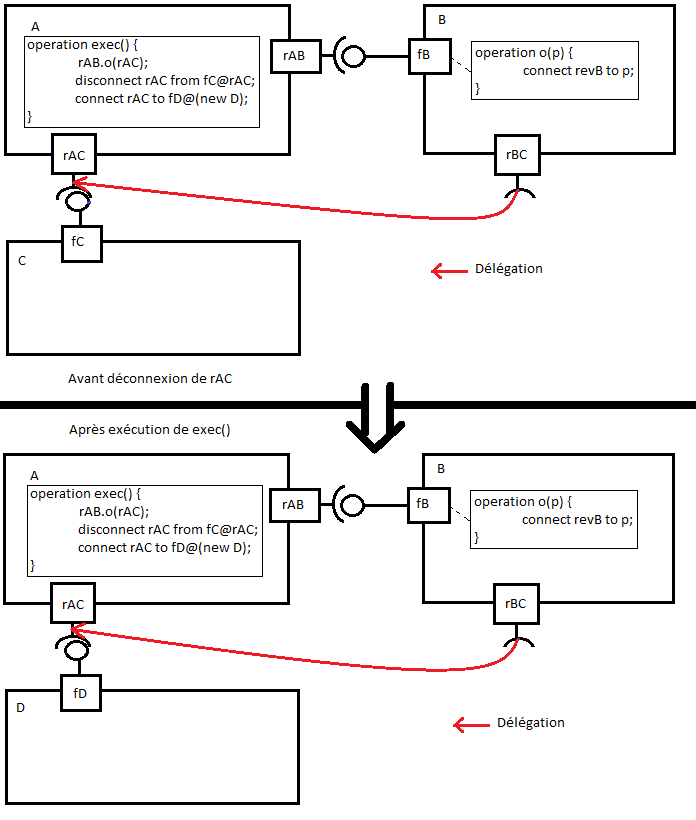
\includegraphics[scale=0.7, keepaspectratio=true]{exempleRequis.png}
\caption{Exemple lors d'un passage d'un port requis en argument à \texttt{o}}
\label{exempleRequis}
\end{figure}
On remarque que lors de la déconnexion de \texttt{rAC} à \texttt{fC}, \texttt{rBC} a aussi perdu son accès à \texttt{fC}. \texttt{rBC} obtient l'accès à \texttt{fD} grâce à la délégation.\\
Le passage d'un port requis en argument est comparable au type de paramètre suivant en C++.

\newpage

\begin{lstlisting}[language=C++, caption=Equivalent en C++ d'un passage de port requis en paramètre de o]
void B::o(Port& p) {
    this->rBC = p;  
}
\end{lstlisting}
Cependant la délégation ne possède pas d'équivalent direct en C++. Dans la figure~\ref{exempleRequis}, \texttt{rBC} ne peut pas modifier la connexion entre \texttt{rAC} et \texttt{fC}. Il peut seulement se déconnecter de \texttt{rAC} (\texttt{this->rBC=NULL} en C++).

\subsection{Qui choisit le mode de passage ?}

Un composant ne peut pas anticiper son utilisation. Il ne peut donc pas anticiper comment il sera connecté à d'autres composants. Il est donc préférable que les composants ne choisissent que leurs connexions lors de l'initialisation et laissent leur conteneur choisir comment ils seront connectés à l'extérieur.\\
De plus si un composant \texttt{A} connecté à \texttt{C} donne accès à \texttt{C} à un composant \texttt{B}, \texttt{A} devrait pouvoir choisir comment la connexion doit s'effectuer.\\
Cependant, il peut exister des cas particuliers dans lesquels l'exécution de l'opération de \texttt{B} ne peut pas fonctionner dans tous les cas. Il faut donc laisser un moyen à \texttt{B} de contraindre le type des arguments.

Le choix du type de connexions créées par une opération \texttt{o} impliquant ses arguments est laissé à l'appelant de \texttt{o}. Néanmoins, dans la signature de l'opération, il est possible de restreindre le type des arguments.


\subsection{Conséquence : Il faut les deux modes de passages}
Le passage d'un port fourni en paramètre possède l'inconvénient de créer des architectures peu réactives aux changements. En effet dans l'exemple de la figure~\ref{exempleFourni}, lors du remplacement du composant C par un composant \texttt{D} par \texttt{A}, la modification n'est pas prise en compte par \texttt{B}.\\
Au contraire, dans le passage d'un port requis, \texttt{rBC} reste toujours connecté au port connecté à \texttt{rAC} par délégation. Cela crée donc une architecture qui peut être modifiée plus facilement.\\
Il existe des cas pour lesquels le second mode de passage d'argument ne convient pas. La figure~\ref{arrayConnexion} propose un exemple de cas où la délégation possède un comportement incompatible avec ce que l'on veut faire. Dans cet exemple, \texttt{A} invoque deux fois l'opération \texttt{add} de \texttt{B} en passant soit \texttt{value}, soit le port fourni connecté à \texttt{value} en paramètre. Entre ces invocations, A change la connexion de \texttt{value}. Les connexions en rouge sont créées si on appelle l'opération \texttt{add} en passant en paramètre un port requis. Les connexions en bleu sont créées si on appelle l'opération en passant en paramètre un port fourni.\\
\begin{figure}[H]
\centering
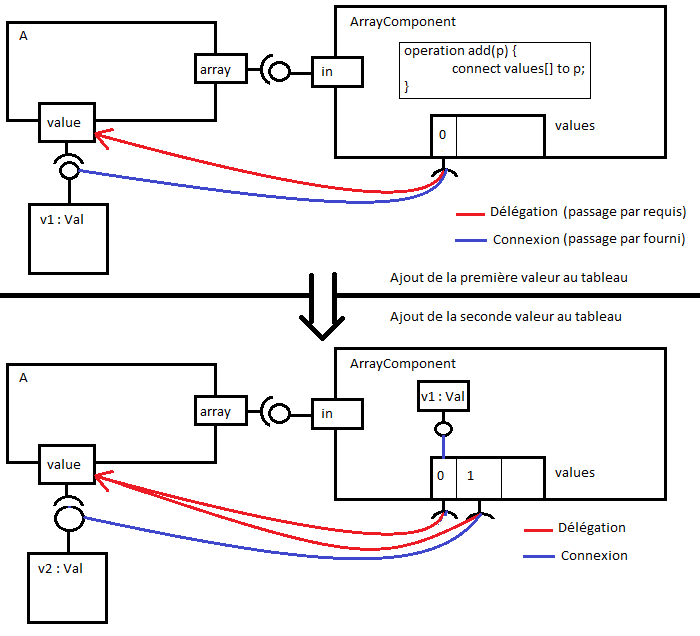
\includegraphics[scale=0.7, keepaspectratio=true]{arrayConnexion.png}
\caption{Cas d'ajout de valeur à un tableau selon que l'on passe un port fourni ou requis en argument de \texttt{add}}
\label{arrayConnexion}
\end{figure}
On remarque que dans le cas où on passe un port requis en argument, la première valeur ajoutée au tableau n'est pas conservée. On obtient à la place deux fois la dernière valeur ajoutée.\\
Il est donc nécessaire de conserver le passage d'argument par port fourni.

\textbf{On doit donc pouvoir passer en arguments d'une opération des ports fournis ou requis.}

\section{Type de retour d'opération}

\subsection{Du point de vue de l'appelant}

\subsubsection{Cas de renvoi d'un composant}
On peut supposer que le retour d'une opération est un composant.\\
Dans ce cas, il n'est pas possible d'enchaîner les opérations. Par exemple, on souhaite exécuter : "\texttt{portRequis.foo().bar();}". On obtiendra une erreur car \texttt{portRequis.foo()} renverra un composant. Or on ne peut invoquer des opérations sur les composants que par un port requis.\\
De plus l'instruction "\texttt{connect monPortRequis to monAutrePortRequis.foo();}" ne fonctionnerait pas également. En effet on ne peut connecter un port qu'à un autre port et non un composant. Ce cas n'est donc pas approprié.

\subsubsection{Cas de renvoi d'un port fourni}
On peut supposer que le retour d'une opération renvoie un port fourni (par exemple \texttt{default}).\\
Dans ce cas, il n'est pas possible d'enchaîner les opérations. Par exemple, on souhaite exécuter : "\texttt{portRequis.foo().bar();}".\\
On obtiendra une erreur car \texttt{portRequis.foo()} renverra un port fourni. Or on ne peut invoquer des opérations que sur des ports requis.\\
Si l'on veut faire cela, il ne faut pas renvoyer directement un port fourni.

\subsubsection{Cas de renvoi d'un port requis}

\label{returnrequisnew}

Le dernier cas de type de retour d'opération possible est de renvoyer un port requis.\\
Dans ce cas l'appelant peut enchaîner les invocations d'opérations car on peut appeler des opérations sur les ports requis.\\
En supposant que l'on accepte la syntaxe "\texttt{connect <portRequis> to <portRequis>}", on peut alors écrire : "\texttt{connect monPortRequis to monAutrePortRequis.foo();}". Cela créera une délégation de \texttt{monPortRequis} vers le résultat de  \texttt{monAutrePortRequis.foo()}.\\
L'appel à \texttt{new()} ne pose également plus de problème. L'exécution de "\texttt{connect monPortRequis to portCible@(ComposantCible.new());}" est possible car : 
\begin{itemize}
\item \texttt{ComposantCible.new()} renvoie un port requis.
\item \texttt{portCible@portRequis} renvoie le port fourni nommé \texttt{portCible} du composant connecté au port requis \texttt{portRequis}.
\item \texttt{connect monPortRequis to portFourni} crée une connexion classique.
\end{itemize}
L'invocation d'une opération peut donc renvoyer un port requis.

Les retours d'opérations (vus par l'appelant) sont des ports requis.



\subsection{Du point de vue du receveur courant}
Nous avons vu que les opérations renvoyaient des ports requis à l'appelant. Maintenant nous devons nous demander ce que renvoie l'exécution d'une opération. C'est à dire de quel type peut être \texttt{x} dans l'instruction "\texttt{return x;}".

\subsubsection{Cas d'un composant}
Dans le cas où on cherche à renvoyer un composant, on se retrouve confronté à un problème.\\
L'appelant attend un port requis. Il faut donc renvoyer un port requis que possède le composant. Or on ne peut pas déterminer quel port choisir automatiquement car il peut exister des composants sans port requis externe.\\
Il n'est donc pas possible de renvoyer un composant.

\subsubsection{Cas d'un port fourni}
Dans le cas où on cherche à renvoyer un port fourni, l'appelant attend un port requis. Il est donc nécessaire de faire une instruction implicite supplémentaire. \\
On propose de connecter le port fourni à renvoyer à un nouveau port requis sans nom, possédé par aucun composant. C'est ce port requis \textbf{anonyme} qui serait reçu par l'appelant.\\
Cette solution peut donc fonctionner mais reste complexe.\\
On peut aussi supposer que dans le cas où on écrit "\texttt{return <portRequis>;}", on renvoie en réalité le port fourni au port requis spécifié. Cela permet de renvoyer tout port fourni connecté à un port requis (ou à un retour d'opération).\\
Dans le cas où on stocke la valeur retournée par une opération, on obtient le cas représenté par la figure~\ref{renvoiFourni}.\\
\begin{figure}[H]
\centering
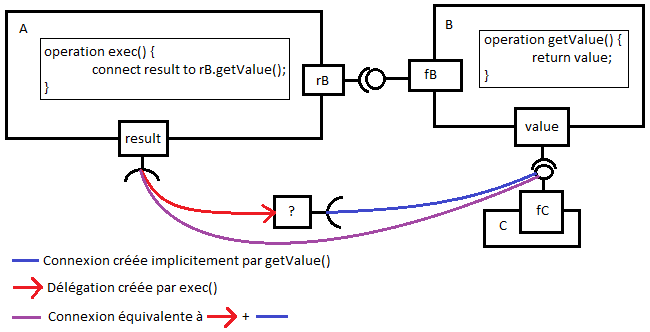
\includegraphics[scale=0.7, keepaspectratio=true]{renvoiFourni.png}
\caption{Cas de renvoi d'un port fourni connecté à un port requis}
\label{renvoiFourni}
\end{figure}
Lors de l'exécution de "\texttt{return value}" dans \texttt{getValue()}, l'interpréteur crée un port requis anonyme (sans nom et attaché à aucun composant) connecté à \texttt{fC} et le renvoie à \texttt{A} (connexion bleue). L'instruction de \texttt{exec()} consiste alors en une connexion requis-requis, donc une délégation de \texttt{result} vers le port anonyme (délégation rouge).\\
On peut réduire le nombre de connexions en simplifiant par une seule connexion entre \texttt{result} et \texttt{fC} (connexion violette). Pour cela il faut modifier l'implémentation de l'opération \texttt{connect} dans les ports requis dans le cas où on cherche à créer une délégation vers un port requis anonyme.\\
Ce cas de figure est équivalent au cas expliqué dans la section~\ref{passageFourni}. En effet on a les propriétés présentes dans les connexions classiques.\\
Cette solution est très similaire au retour de méthode en Java.

\subsubsection{Cas d'un port requis}
Nous avons vu que le retour d'une opération était un port requis pour l'appelant. La solution la plus simple est donc de pouvoir renvoyer un port requis côté receveur courant.\\
Ainsi contrairement au cas précédent, on n'a plus besoin de passer par un port requis anonyme puisqu'on renvoie un port requis.\\
Si on reprend l'exemple proposé dans le cas précédent avec un retour par port requis, on obtient la figure~\ref{renvoiRequis}.\\
\begin{figure}[H]
\centering
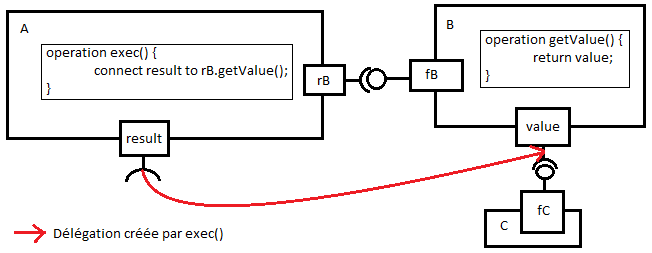
\includegraphics[scale=0.7, keepaspectratio=true]{renvoiRequis.png}
\caption{Cas de renvoi d'un port requis connecté à un port requis}
\label{renvoiRequis}
\end{figure}
On remarque que la connexion entre \texttt{result} et \texttt{fC} est similaire, et donc possède les mêmes propriétés, que celle présente dans la section~\ref{passageRequis}. En effet la délégation permet d'obtenir les mêmes propriétés.\\
Cette solution pose un problème. Car c'est \texttt{B} qui choisit ce qu'il renvoie. Il peut donc modifier la connexion impliquant \texttt{value}, qui modifiera par la délégation la connexion de \texttt{result}. Or \texttt{B} ne doit pas pouvoir anticiper comment il sera utilisé. Il y a donc une contradiction.\\
C'est pourquoi nous pensons que ce mode de connexion n'est pas utilisable.

\subsubsection{Renvoyer un port fourni}
D'après les paragraphes précédents, on peut dire qu'il est préférable de renvoyer un port fourni. Celui-ci sera alors connecté à un port requis anonyme et passé à l'appelant.

Il peut être intéressant pour des questions de performances d'éviter les délégations d'un port requis vers un port anonyme. Lorsqu'un cas pareil se présente (voir exemples~\ref{renvoiFourni} et~\ref{renvoiRequis}), la connexion est effectuée entre le port requis et le port fourni connecté au port anonyme. Ce dernier est ensuite détruit.

\subsection{Cas particulier : l'opération new()}
Afin de créer une nouvelle instance de composant, on invoque l'opération \texttt{new} sur son descripteur.\\
D'après \ref{returnrequisnew} , \texttt{new()} renvoie un port requis anonyme connecté à un port fourni \texttt{default} du composant nouvellement créé.
Ce port anonyme possède les mêmes propriétés qu'un port requis nommé. Il peut, par exemple, servir comme tout autre port à identifier le composant auquel il est connecté. Cela est notamment nécessaire pour connecter un port fourni spécifique d'un nouveau composant à un de ses ports requis. 

\begin{lstlisting}[language=Compo, frame=single, caption=]
connect monPortRequis to portFourniCible@(DescripteurCible.new());
\end{lstlisting}

\clearpage

\section{Les services et l'encapsulation}

\subsection{Modification de la connexion entre deux composants distants}
\label{serviceEncapsulationRef}
Dans un service, il est actuellement possible de modifier une connexion d'un composant distant au travers d'autres composants.
Cette utilisation constitue un abus du langage COMPO et ne devrait pas être permis. En effet, cela constitue une infraction au principe d'encapsulation. 

Il est possible pour un composant d'utiliser la couche réflexive pour connaître les composants qui sont connectés à un port et ainsi pouvoir modifier des connexions à l'extérieur de lui-même. 

Sinon, il faut connaître l'architecture du programme, un exemple de cette déconnexion distante est donnée en annexe \ref{deconnexiondistante}.

\subsection{Modification de connexion d'un port externe}

Prenons un compteur simple représenté par la figure \ref{compteursimple}. Ajoutons lui un service \texttt{foo} qui modifie la connexion d'un port externe comme dans \ref{compteurservicefoo}.

\begin{figure}[H]
\centering
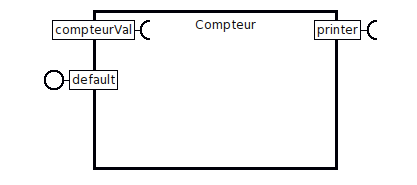
\includegraphics[scale=0.7, keepaspectratio=true]{compteursimple}
\caption{Schéma d'un compteur extrait de \texttt{Compobrowser2}}
\label{compteursimple}
\end{figure}

\begin{lstlisting}[language=Compo, frame=single, caption=Exemple d'un service dans un composant compteur,label=compteurservicefoo]
service foo {
    connect printer@self to default@(MorphPrinter.new());
}
\end{lstlisting}

Cet exécution permet de connecter le port requis externe \texttt{printer} à un nouveau \texttt{printer}, dans ce cas un \texttt{MorphPrinter}

Quand on exécute le programme, le résultat ne sera pas celui attendu car le \texttt{printer} utilisé ne sera pas celui défini par l'architecte lors de la création du programme. En effet, le \texttt{printer} connecté sera modifié lors de l'exécution du service \texttt{foo}.

\textbf{Nous pensons qu'il ne devrait pas être possible pour un composant de modifier une connexion sur un port externe dans un service}

Pour cela, on pourrait interdire l'utilisation du mot clé \texttt{@} dans les services si le port est un port externe.

\section{Le typage en COMPO}
Actuellement, COMPO est un langage à typage dynamique. Il peut être intéressant de voir les points forts et points faibles des typages possibles en COMPO afin d'en préconiser celui que nous estimerons le plus intéressant.

\subsection{Le typage dynamique}
Le typage dynamique permet de programmer rapidement avec une syntaxe minimale des programmes complexes.\\
Dans COMPO ces points forts sont
\begin{itemize}
\item Syntaxe minimale : ne pas préciser les types pour les variables ou les signatures d'opérations permet de garder une syntaxe minimale et lisible.
\item Retrait des problèmes du polymorphisme : grâce au typage dynamique, il est possible de connecter un port requis à un port fourni peu importe d'où il vient.
\end{itemize}

Néanmoins les inconvénients sont similaires à ceux que l'on peut retrouver en langage à objets à typage dynamique : 
\begin{itemize}
\item Code peu lisible : l'absence de typage implique qu'il est difficile de reprendre un code créé par une autre personne. Il est difficile de savoir quel type d'argument est demandé par une opération par exemple.
\item Vérification de la cohérence du code à l'exécution : on ne peut anticiper les erreurs liées au typage à la compilation. On est obligé de faire des tests afin de vérifier que le code est cohérent.
\end{itemize}

\subsection{Le typage statique}
Le typage statique propose des codes plus complexes mais aussi plus précis.\\
L'utilisation du typage statique en COMPO permettrait
\begin{itemize}
\item Vérification de la cohérence du code à la compilation : le typage statique permettrait de vérifier à la compilation d'un descripteur si les connexions sont cohérentes par exemple.
\item Signatures d'opérations plus lisibles : ajouter des types aux arguments et au retour des opérations, permettrait d'expliciter ce qu'attend l'opération pour fonctionner.
\end{itemize}

Cependant cette solution possède des inconvénients : 
\begin{itemize}
\item Typage très contraignant sur l'origine des composants : le fait de typer statiquement les arguments ou les ports, restreint l'origine des composants. En effet en typage statique il faut que le type d'une variable et ce qu'elle contient possède une relation d'héritage (polymorphisme). Cette relation d'héritage implique qu'il est difficile de mettre en relation des composants d'origines diverses.
\item Code plus lourd : COMPO cherche à rester minimaliste et l'ajout du typage statique rendrait la syntaxe beaucoup plus lourde (surtout sur les signatures d'opérations).
\end{itemize}

\clearpage

\subsection{Notre solution : le typage par interface}
Typer les arguments d'opérations par une liste d'opérations comme pour les ports. On peut retrouver ce type de vérification de compatibilité dans certains ADL comme DEDAL~\citep{dedal}.\\
On obtiendrait ainsi : 
\begin{itemize}
\item Un code lisible pour les opérations : l'ajout de ce typage permet de mieux comprendre ce dont a besoin l'opération pour fonctionner.
\item Une vérification de la cohérence du code à la compilation : il est possible de vérifier la compatibilité des connexions et des passages d'arguments à la compilation en comparant les interfaces (anonymes ou nommées).
\item Retrait des problèmes liés au polymorphisme : il n'y a plus de problème lié aux relations d'héritage dans le typage par interface puisqu'on compare la liste des signatures d'opérations.
\end{itemize}

\chapter{Nos contributions au langage COMPO}

Nous présentons dans ce chapitre une partie de nos contributions.

\section{Connexion à des littéraux}

Il n'était pas possible de connecter un port directement à un littéral. Nous souhaitons donc rajouter cette possibilité. Cela permet au développeur de facilement connecter un port à un nombre (entier ou à virgule). On peut également se connecter directement à une chaîne de caractère. 

Pour faciliter l'implémentation, nous avons ajouté de manière temporaire le mot clef \texttt{rockonnect}. Le littéral \textit{parsé} est connecté au port par l'intermédiaire de la création d'un \texttt{LiteralAtomicPort}, une spécialisation de \texttt{AtomicPort}

Par la suite, nous avons fusionner le mot clef \texttt{rockonnect} et \texttt{connect}. Il est donc désormais possible pour un développeur d'utiliser le mot clé \texttt{connect} pour se connecter aux littéraux. Le mot clé \texttt{rockonnect} a depuis été supprimé.

\begin{lstlisting}[language=Compo, frame=single, caption=Syntaxe d'une connexion à un littéral]
connect compteurVal@self to 1;
connect compteurVal@self to 3.14;
connect compteurVal@self to 'Hello World';
\end{lstlisting}


\section{Enchainement des \texttt{connect} sur un même port}

Il n'était jusqu'à lors pas possible d'enchaîner les \texttt{connect} sur un même port. Seul le premier \texttt{connect} était prit en compte. Il fallait utiliser entre chaque modification le mot clé \texttt{disconnect}.


\subsubsection{Implémentation du \texttt{disconnect}}

Le mot cléf \texttt{disconnect} existait déjà dans COMPO mais n'était pas implémenté. Nous avons donc ajouté la logique métier. Celui-ci permet de couper une connexion entre deux ports.

\begin{lstlisting}[language=Compo, frame=single, caption=Syntaxe d'une déconnexion]
disconnect compteurValSyndicat@self from default@compteurValSyndicat
\end{lstlisting}

Cet ajout va nous permettre de pouvoir par exemple modifier la valeur d'un compteur.

L'utilisation de ce mot clé est problématique dans la mesure où il nécessaire de savoir si un port est connecté à quelque chose ou pas avant de pouvoir le connecter à un autre composant. 

\subsubsection{Ajout du \texttt{disconnect} automatique lors d'une connexion}

Nous souhaitons que l'utilisateur puisse modifier une connection sans utiliser le mot clé \texttt{disconnect}. Nous avons donc rajouté l'appel au \texttt{disconnect} de manière automatique avant chaque connexion.

\begin{lstlisting}[language=Compo, frame=single, caption=Syntaxe d'une connexion entre un port et un littéral]
connect compteurVal@self to 1;
connect compteurVal@self to 2;
connect compteurVal@self to 3;
\end{lstlisting}

Cet enchaînement permet de se connecter au port \texttt{1}, \texttt{2}, puis \texttt{3}. Cet abstraction permet à l'utilisateur de ne pas utiliser le mot clé \texttt{disconnect} entre chaque opération. Celui-ci sera fait automatiquement par COMPO. 

\section{Nouvelle syntaxe d'une connexion}

A la manière de l'affectation SmallTalk, nous avons implémenté une nouvelle syntaxe de connexion. Nous avons choisi $>>>$ qui peut donc remplacer le traditionnel \texttt{connect to}. Cette syntaxe moins verbeuse permet également de s'abstraire du \texttt{@self}.

\begin{lstlisting}[language=Compo, frame=single, caption=Comparaison entre l'ancienne et la nouvelle syntaxe d'une connexion]
"Nouvelle syntaxe"
compteurVal >>> 1;

"Ancienne syntaxe"
connect compteurVal@self to 1;
\end{lstlisting}

Les deux syntaxes sont actuellement valides pour définir une affectation.

\section{Ajout de primitives SmallTalk en COMPO}

COMPO étant basé sur SmallTalk, il peut être intéressant pour un développeur de pouvoir utiliser des primitives.
Nous avons donc rajouté une syntaxe qui permet d'indiquer à l'analyseur syntaxique que ce qui suit est une primitive SmallTalk. 

\begin{lstlisting}[language=JAVA, frame=single, caption=Syntaxe d'une primitive smalltalk en COMPO]
<! 
    Transcript crShow: 'Hello'.
>
\end{lstlisting}

\section{Définir un \texttt{service} avec le mot clé \texttt{operation} }

Lors de discussions avec des non initiés au langage COMPO, l'utilisation du mot clé \texttt{service} comportait des ambiguïtés. Pour faciliter la compréhension du langage, nous avons rajouté le mot clé \texttt{operation} pour définir un service. Ce dernier permet de faire le paralléle plus facilement avec les autres langages.

\begin{lstlisting}[language=COMPO, frame=single, caption=Syntaxe d'une opération en COMPO]
operation foo() {
    "TODO"
}
\end{lstlisting}

Il est donc possible d'utiliser les deux mots clés dans le langage pour définir un service.


\section{Vérification de compatibilité lors des connexions}

Nous avons donc rajouté une vérification des compatibilités de connexions.

\subsubsection{A la compilation}

Quand le développeur fait un \textit{accept}, une erreur lui indique s'il a fait une connexion entre deux composants incompatibles.

\begin{lstlisting}[language=Compo, frame=single, caption=Exemple de connexion incorrecte]
internally requires {
    myPort : { foo() };
}
architecture {
    connect myPort@self to default@(MyComponent.new());
}
\end{lstlisting}

Si \texttt{MyComponent} n'implémente pas de méthode \texttt{foo}, lors du \texttt{accept}, le développeur aura le message d'erreur suivant : 

\begin{lstlisting}[language=Compo, frame=single, caption=Message d'erreur lorsque les interfaces sont incompatibles]
Incompatible interfaces between myPort@self and default@(MyComponent.new());
\end{lstlisting}

\subsubsection{A l'exécution}

Une seconde vérification de comptabilité est faite à l'exécution car il est possible d'effectuer un \texttt{connect} dans un service.

\begin{lstlisting}[language=Compo, frame=single, caption=Extrait d'un descripteur Compteur]
Descriptor Compteur extends Component
{
	requires {
		printer: { foo(); };
	}
}
\end{lstlisting}

Le compteur a besoin d'un \texttt{printer} qui possède une méthode \texttt{foo}.


\begin{lstlisting}[language=Compo, frame=single, caption=Service qui lancera une exception lors de son invocation]
Descriptor Program extends Component
{
	service init() {
		connect printer@self to default@(Printer.new());
	}
}
\end{lstlisting}

L'exécution de ce service \textit{init} plantera à l'exécution si \texttt{Printer} ne possède pas de service \texttt{foo}. L'invocation du service \texttt{foo} aura donc pour conséquence d'arrêter l'exécution et de déclencher l'erreur suivante.

\begin{lstlisting}[language=Compo, frame=single, caption=Message d'erreur lorsque les interfaces sont incompatibles]
Incompatible interfaces between printer and printing
\end{lstlisting}



\section{Retour par port requis ou fourni}

\subsubsection{Par port requis}
Nous souhaitons que le développeur puisse chaîner les opérations. Or, les invocations d'opérations ne peuvent se faire que sur des ports requis. Il faut donc qu'une opération rende un port requis.

Le code suivant permet de récupérer le composant \texttt{Printer} connecté au compteur et d'invoquer le service \texttt{print()} directement.
\begin{lstlisting}[language=JAVA, frame=single, caption=Syntaxe d'un chaînage d'invocation en COMPO]
compteur.getPrinter().print('Hello');
\end{lstlisting}



\begin{lstlisting}[language=COMPO, frame=single, caption=Syntaxe de retour d'un port requis en COMPO]
service foo() {
    return !portInterne;
}
\end{lstlisting}

Cette syntaxe permet de retourner un port requis directement.


\subsubsection{Par port fourni}
Il peut être intéressant de retourner un port fournis dans le cas où l'on souhaite réutiliser le résultat d'un service.


\begin{lstlisting}[language=COMPO, frame=single, caption=Syntaxe de retour d'un port founis en COMPO]
service foo() {
    return 1;
}
\end{lstlisting}

Lors de la définition d'un service, un composant peut choisir de retourner directement un port requis.
Nous donnons en Annexe \ref{annexeretourcomparaison} un exemple pour montrer la différence de comportement entre ces deux modes de retour.

\section{Précisions du type de retour dans la signature d'une opération}
Nous avons ajouté une syntaxe qui garanti le retour d'un port requis ou fourni par les mots clés \texttt{:req} et \texttt{:pro}.\\
Cette syntaxe a, avant tout pour but, de spécifier le comportement d'une opération sous la forme d'une assertion en précisant si elle renvoie un port requis ou fourni. Si l'assertion n'est pas vérifiée, une exception est levée.

\begin{lstlisting}[language=COMPO, frame=single, caption=Syntaxe du typage de retour d'opération]
operation foo() :pro {
    return 1;
}
operation bar() :req {
    return !aRequiredPort;
}
\end{lstlisting}

\section{Passage d'arguments par fourni ou requis}

Nous avons implémenté la possibilité de choisir le mode de passage. Si l'on précède la variable par un \texttt{!}, cela revient à passer le port directement. Le choix du mode de passage est totalement transparent pour le receveur.

\begin{lstlisting}[language=COMPO, frame=single, caption=Syntaxe du passage par founis en COMPO]
a.foo(var);
\end{lstlisting}

\begin{lstlisting}[language=COMPO, frame=single, caption=Syntaxe du passage par requis en COMPO]
a.foo(!var);
\end{lstlisting}

Imaginons que le composant \texttt{A} enregistre cette \texttt{var} grâce à la méthode \texttt{foo}. Si on change ce qui est connecté à mon port \texttt{var} à l'extérieure de \texttt{A} il sera également modifié dans \texttt{A}.

Nous donnons en Annexe \ref{passagereqprovider} un exemple pour montrer la différence de comportement entre ces deux modes de passages.

\chapter{Conclusion}

\section{Le langage COMPO}

COMPO est actuellement l'un des seuls langages de programmation orienté composants qui soit réflexif. Cette spécificité nous a amené à étudier son fonctionnement.\\
COMPO étant à l'état de prototype, nous avons proposé des améliorations possibles du langage.\\
Nous en sommes arrivés aux conclusions suivantes.

\subsubsection{Analyse des connexions}
Il existe trois modes de connexion possibles en COMPO : 
\begin{description}
\item[Connexion standard]C'est une connexion entre un port requis et un port fourni. Ces connexions ne sont pas impactées par des modifications de connexions extérieures.
\item[Délégation]C'est une connexion entre deux ports requis ou deux ports fournis. Une délégation peut être impactée par des modifications de connexions extérieures. On peut rendre une architecture plus simple à maintenir par des délégations.
\item[Connexion partagée]Cette connexion n'est pas implémentée actuellement dans COMPO. Il s'agit d'une connexion entre plusieurs ports requis vers un port fourni. Lorsque le possesseur d'un des ports requis modifie sa connexion, la modification est transmise aux autres connexions.
\end{description}

\subsubsection{Passage d'arguments}
Nous avons vu qu'il était possible de passer en argument un port fourni ou un port requis. Selon le mode de passage choisi (par l'appelant), le comportement de l'opération côté appelé change.

\subsubsection{Type de retour d'opération}
Nous avons vu qu'il existait deux modes de retour possible pour les opérations du point de vu du receveur courant : retour d'un port requis ou d'un port fourni.\\
Du côté de l'appelant, ce dernier ne reçoit que des ports requis afin de pouvoir enchaîner les invocations d'opérations.

\subsubsection{Les services et l'encapsulation}
Nous avons mis en évidence un problème lié à l'accès à un port distant par l'opérateur \texttt{@} de COMPO dans les opérations.\\
Cela brise l'encapsulation des composants. Cependant nous avons précisé qu'il s'agit d'un cas particulier. En effet pour accéder à un port distant, le composant doit avoir conscience de l'architecture globale du programme. Il peut en avoir conscience par introspection.

\subsubsection{Le typage en COMPO}
Nous avons réfléchi sur le mode de typage que devrait adopter COMPO. Actuellement en typage dynamique, nous avons conclu qu'il était préférable d'opter pour un typage "hybride" entre le typage statique et le typage dynamique. Ce mode intermédiaire ne vérifierait la compatibilité qu'au niveau des signatures d'opérations que doit fournir (ou requiert) un port fourni (ou un port requis).

\section{Nos contributions}

Nous avons souhaité contribuer au langage COMPO pour améliorer sa syntaxe, mais également ses possibilités. Voici un rapide résumé des apports développés au sein de ce projet.

\subsubsection{Connexion à des littéraux}
Nous avons rajouté la possibilité de connecter un port directement à un littéral SmallTalk (nombre ou chaîne de caractère).\\
Pour cela nous avons créé un nouveau type de port atomique fourni nommé \texttt{LiteralAtomicPort} héritant de \texttt{AtomicPort}.

\subsubsection{Enchaînement des connexions sur un même port}
Nous avons permis l'enchaînement des connexions sur un même port. Auparavant, lorsqu'un port était déjà connecté, il ne se connectait pas au nouveau port demandé tant qu'il n'était pas au préalable déconnecté.

\subsubsection{Nouvelle syntaxe d'une connexion}
Nous avons pu remarquer qu'une connexion était très similaire à une affectation dans d'autres langages comme le C. Nous avons donc augmenté la syntaxe des connexions afin de montrer visuellement ce lien tout en les distinguant par l'opérateur $>>>$.

\subsubsection{Ajout de primitives SmallTalk en COMPO}
Afin de pouvoir ultérieurement améliorer les opérations de la couche réflexive de COMPO, il était nécessaire de pouvoir utiliser du code SmallTalk directement en COMPO. Nous avons donc augmenté la syntaxe afin de créer de telles sections de code.

\subsubsection{Définir un \texttt{service} avec le mot clé \texttt{operation}}
Nous pensons qu'il est nécessaire de changer le mot clé \texttt{service} par le mot clé \texttt{operation} pour éviter les confusions avec les \textit{webservices} (complètement différents).

\subsubsection{Vérification de compatibilité lors des connexions}
Afin d'implémenter le typage "hybride" proposée dans nos réflexions sur le typage de COMPO, nous avons implémenté une vérification de compatibilité des connexions.\\
On a ainsi implémenté une vérification à la compilation pour la clause \texttt{architecture} du programme. Une autre vérification est réalisée à l'exécution pour les connexions effectuées dans les opérations.

\subsubsection{Retour par port requis ou fourni}
Nous avons implémenté la possibilité de renvoyer un port fourni connecté à un port requis ou directement un port requis grâce à l'utilisation du mot clé "\texttt{!}".\\
L'appelant reçoit dans tous les cas un port requis (pouvant être anonyme si le receveur courant de l'opération invoquée renvoie un port fourni) afin de pouvoir enchaîner les invocations d'opérations.

\subsubsection{Précisions du type de retour dans la signature d'une opération}
Nous avons ajouté une syntaxe optionnelle faisant office d'assertion sur le type de retour d'une opération. En utilisant les mots clés \texttt{:req} ou \texttt{:pro} dans la signature d'une opération, on précise ce qu'elle renvoie. 

\subsubsection{Passage d'arguments par fourni ou requis}
De la même manière que pour le retour par port requis ou fourni, l'opérateur "\texttt{!}" nous a permis de pouvoir passer en argument des ports fournis ou des ports requis. Selon le mode de passage choisi, le comportement de l'opération en est modifiée.

\section{Difficultés rencontrées}

\subsubsection{Le code généré}

Une partie du langage COMPO est basé sur du code généré. Lors de nos ajouts, cette spécificité nous a très vite posé problème. En effet, lorsque l'on fait une modification, le code est à nouveau généré. Or, certaines portions du code généré avait été modifiées "à la main" pour effectuer des correctifs. Lorsque nous avons essayé de modifier le code de base, celui généré ne comportait plus les correctifs.

\subsubsection{Le retour par requis}
Pour renvoyer un port requis dans une opération et non ce à quoi il est connecté, nous avions pensé dans un premier temps à rajouter un opérateur \texttt{:req} dans la signature du service.\\
Ci-dessous, on suppose que le composant \texttt{Cpt} possède un port requis \texttt{A}, connecté à un autre composant. Cet exemple renvoie le port requis \texttt{A} et non ce à quoi il est connecté.
\begin{lstlisting}[language=COMPO, frame=single, caption=Syntaxe d'une opération avec \texttt{:req} en COMPO]
operation foo() :req {
    return A;
}
\end{lstlisting}
On a remarqué que l'ajout du \texttt{!} par la suite posait problème car les deux opérateurs peuvent répondre à la même demande. Nous avons donc modifié \texttt{:req} pour le transformer en une assertion. Si \texttt{foo()} ne retourne pas un port requis, le programme lève une exception.

\section{Perspectives}

Notre problématique étant complexe, la solution qui y répond est complexe aussi. Notre étude nous a permis de comprendre les difficultés en question. Ainsi, les perspectives d’avenir de notre projet sont multiples et variées.

\subsubsection{Augmenter la vérification de compatibilité}
Actuellement, la vérification de compatibilité ne fonctionne que sur les interfaces anonymes.\\
Le port \texttt{default} généré sur tous les composants est toujours attribué avec une interface "*". Hors une interface nommée est l'interface du port \texttt{default} du composant de même nom (donc "*").\\
Il faudrait donc modifier comment est générée l'interface du port \texttt{default} afin de pouvoir avoir une vérification de compatibilité dans tous les cas.

\subsubsection{Implémenter la connexion partagée}
Nous avons vu dans~\ref{connexionPartageeRef} qu'il pourrait exister un troisième type de connexion : la connexion partagée.\\
Elle n'est pas implémentée dans COMPO actuellement. On peut la simuler mais il n'y a pas de raccourci syntaxique pour en créer une automatiquement.\\
L'ajout d'une telle connexion demanderait d'augmenter la syntaxe du \texttt{parseur}, et d'ajouter de nouveaux types de ports requis.

\subsubsection{Implémenter les opérations de la couche réflexive}
COMPO est un langage réflexif. Cependant les opérations de la couche réflexive ne sont pas toutes implémentées. On effectue actuellement l'introspection directement en SmallTalk en suivant les relations créées par COMPO.\\
Ces opérations ne poseraient pas de problèmes pour être implémentées grâce au fait qu'on puisse écrire du code SmallTalk directement dans une opération par la syntaxe \texttt{<! ... >}.

\subsubsection{Interdire l'accès à un port distant auquel on n'est pas connecté}
On a vu dans~\ref{serviceEncapsulationRef} que l'accès à un port distant auquel on n'est pas connecté pouvait poser problème dans une opération. Il peut être intéressant d'interdire ces accès par le mot-clef \texttt{@} et forcer l'utilisation d'opérations servant d'accesseurs.

\subsubsection{Extraire COMPO de Pharo}
Actuellement, COMPO fonctionne en environnement fermé dans Pharo. Pouvoir s'extraire de cet environnement pourrait permettre une exportation plus simple et une utilisation d'outils externes plus élaborés. Par exemple on pourrait utiliser COMPO dans Eclipse et obtenir toute la puissance d'un tel environnement de développement.

\bibliographystyle{plain}

\bibliography{references}

\begin{appendices}
\appendixpage
\noappendicestocpagenum
\addappheadtotoc

\chapter{Parallèle entre COMPO et JAVA pour une délégation}

\chaptermark{Comparaison COMPO / JAVA}

\label{Annexe A}

Nous allons réaliser en COMPO puis en Java un exemple de délégation. On prend un cameraman, un interviewer et une personne qui est interviewée. Le but est que le cameraman filme en permanence la personne que l'interviewer est en train d'interroger. L'interviewer va donc commencer à discuter avec une \texttt{ExpressivePerson} puis une \texttt{SadPerson}". Le but est que le cameraman et l'interviewer aient toujours le \textit{focus} sur la même personne.

\subsubsection{COMPO}
\begin{lstlisting}[language=Compo, frame=single, caption=Cameraman]
Descriptor Cameraman extends Component {

    provides {
        listen: { listen(txt) };
    }
    
    requires {
        chat: { chat(txt); };
    }
    
    architecture {
        connect chat@self to chat@(Interviewer.new());
    }
    
    service listen() {
        Transcript.show('The cameraman is listening... ');
        Transcript.crShow(chat@self.chat());
    }
}
\end{lstlisting}

\newpage

\begin{lstlisting}[language=Compo, frame=single, caption=Interviewer]
Descriptor Interviewer extends Component {

    provides {
        interview: { interview(txt) };
    }
    
    requires {
        chat: { chat(txt); };
    }
    
    architecture {
        connect chat@self to chat@(SadPerson.new());
    }
    
    service interview() {
        Transcript.show('Hello, what do you think? ');
        Transcript.crShow(chat@self.chat());
    }
}
\end{lstlisting}

\begin{lstlisting}[language=Compo, frame=single, caption=SadPerson]
Descriptor SadPerson extends Component {

    provides {
        chat: { chat(txt); };
    }
    
    service chat(txt) {
        return 'You will fail your life.';
    }
}
\end{lstlisting}

\begin{lstlisting}[language=Compo, frame=single, caption=ExpressivePerson]
Descriptor ExpressivePerson extends Component {

    provides {
        chat: { chat(txt); };
    }
    
    service chat(txt) {
        return 'I am in love with you.';
    }
}
\end{lstlisting}


\clearpage

\subsubsection{Java}

\begin{lstlisting}[language=Java, frame=single, caption=IChatty]
package compo;

public interface IChatty {
    String chat();
}
\end{lstlisting}

\begin{lstlisting}[language=Java, frame=single, caption=SadPerson]
package compo;

public class SadPerson implements IChatty {
    @Override
    public String chat() {
        return "You will fail your life.";
    }
}
\end{lstlisting}

\begin{lstlisting}[language=Java, frame=single, caption=ExpressivePerson]
package compo;

public class ExpressivePerson implements IChatty {
    @Override
    public String chat() {
        return "I'm in love with you.";
    }
}
\end{lstlisting}

\begin{lstlisting}[language=Java, frame=single, caption=ChattyPointer]
package compo;

public class ChattyPointer<T extends IChatty> {
    private T m_data;

    public T data() {
        return this.m_data;
    }

    public void define(T data) {
        this.m_data = data;
    }
}
\end{lstlisting}

\clearpage

\begin{lstlisting}[language=Java, frame=single, caption=Cameraman]
package compo;

public class Cameraman {
    private IChatty chater;
    private ChattyPointer<IChatty> target;

    public Cameraman() {
        this.chater = null;
        this.target = null;
    }

    public void setChater(IChatty chater) {
        this.chater = chater;
    }

    public void setTarget(ChattyPointer<IChatty> target) {
        this.target = target;
    }

    public void listen() {
        System.out.print("The cameraman is listening... ");
        System.out.println(this.chater.chat());
    }

    public void smartListen() {
        System.out.print("The cameraman is listening... ");
        System.out.println(this.target.data().chat());
    }
}
\end{lstlisting}

\clearpage

\begin{lstlisting}[language=Java, frame=single, caption=Interviewer]
package compo;

public class Interviewer {
    private IChatty chater;
    private ChattyPointer<IChatty> target;

    public Interviewer() {
        this.chater = null;
        this.target = new ChattyPointer<IChatty>();
    }

    public void setChater(IChatty chater) {
        this.chater = chater;
    }

    public void setTarget(IChatty chater) {
        this.target.define(chater);
    }

    public IChatty getChater() {
        return this.chater;
    }

    public ChattyPointer<IChatty> getTarget() {
        return this.target;
    }

    public void interview() {
        System.out.print("Hello, what do you think? ");
        System.out.println(this.chater.chat());
    }

    public void smartInterview() {
        System.out.print("Hello, what do you think? ");
        System.out.println(this.target.data().chat());
    }
}
\end{lstlisting}

\clearpage

\begin{lstlisting}[language=Java, frame=single, caption=Program]
package compo;

public class Program {
    public static void main(String[] args) {
        IChatty sadPerson = new SadPerson();
        IChatty expressivePerson = new ExpressivePerson();

        Interviewer interviewer = new Interviewer();
        Cameraman cameraman = new Cameraman();

        interviewer.setChater(sadPerson);
        cameraman.setChater(interviewer.getChater());

        interviewer.interview();
        cameraman.listen();

        interviewer.setChater(expressivePerson);

        interviewer.interview();
        cameraman.listen();

        System.out.println("Simulation of required");
        interviewer.setTarget(sadPerson);
        cameraman.setTarget(interviewer.getTarget());

        interviewer.smartInterview();
        cameraman.smartListen();

        interviewer.setTarget(expressivePerson);

        interviewer.smartInterview();
        cameraman.smartListen();
    }
}
\end{lstlisting}

\subsubsection{Explication}
L'application Java donnera à l'execution dans la console : \begin{lstlisting}[frame=single, caption=output]
Hello, what do you think? You will fail your life. 
The cameraman is listening... You will fail your life.
Hello, what do you think? I'm in love with you. 
The cameraman is listening... You will fail your life. 
Simulation of required 
Hello, what do you think? You will fail your life. 
The cameraman is listening... You will fail your life. 
Hello, what do you think? I'm in love with you. 
The cameraman is listening... I'm in love with you.
\end{lstlisting}
On utilise en Java un objet qui va servir à garder le lien sur la personne en interview.

\chapter{Compteur de manifestants en COMPO}

Nous avons implémenté en COMPO un exemple de compteur de manifestants. Celui-ci comporte un composant instance de \texttt{Compteur} qui implémente la logique métier et un composant instance de \texttt{Printer} qui affiche la valeur du compteur. Dans un premier temps on met un compteur de la police, on remplace ensuite ce compteur par celui des syndicats.

\begin{figure}[H]
\centering
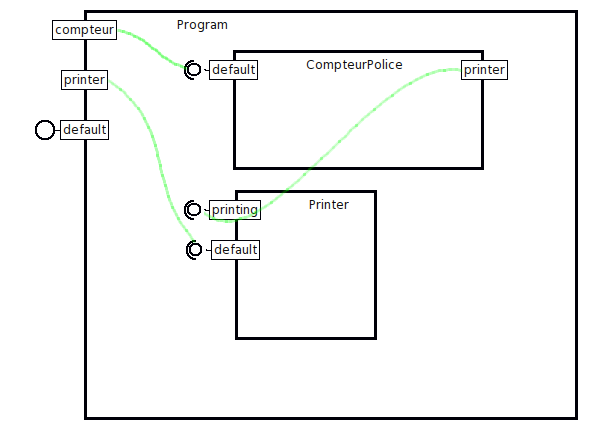
\includegraphics[scale=0.7, keepaspectratio=true]{program}
\caption{Schéma du programme extrait de \texttt{Compobrowser2}}
\label{compteurmanifestant}
\end{figure}

\newpage

\begin{lstlisting}[language=Compo, frame=single, caption=worspace]
|compteur|
compteur := Program.new();
compteur.print();
compteur.incrementer();
compteur.print();
\end{lstlisting}

\begin{lstlisting}[language=Compo, frame=single, caption=output (Avec le \texttt{CompteurPolice})]
0
1
\end{lstlisting}

On remplace le compteur de la police par celui des syndicats. Pour cela, on met en commentaire la ligne 15 et on dé-commente la ligne 16 de \ref{program}. On exécute à nouveau le programme.

\begin{lstlisting}[language=Compo, frame=single, caption=output (Avec le \texttt{CompteurSyndicat})]
0
5
\end{lstlisting}


\begin{lstlisting}[language=Compo, frame=single, caption=Programme utilisant un compteur, label=program]
Descriptor Program extends Component
{
	provides {
		default: {
			incrementer();
			print();
		 };
	}
	internally requires {
		compteur : Compteur;
		printer: Printer;
	}
	architecture {
        connect compteur@self to default@(CompteurPolice.new());
	    "connect compteur@self to default@(CompteurSyndicat.new());"
        connect printer@self to default@(Printer.new());
        connect printer@compteur to printing@printer;
	}
	
	service incrementer() {
		compteur.incrementer();
	}
	
	service print() {
		compteur.showResult();
	}
}
\end{lstlisting}

\newpage
\begin{lstlisting}[language=Compo, frame=single, caption=Compteur de la Police]
Descriptor CompteurPolice extends Component
{
	provides {
		default: {
			 incrementer(); 
			 incrementer(val); 
			 showResult();
		};
	}
	
	internally requires {
			compteurVal : SmallInteger;
	}
	
	requires {
		printer: { print(txt); };
	}
	
	architecture {
	    connect compteurVal@self to 0;
	}
	
	service incrementer(val) {
	    | t |
	    t := compteurVal.asString().asInteger() + val;
	    connect compteurVal@self to t;
	}
	
	service incrementer() {
	    | t |
	    t := compteurVal.asString().asInteger() + 1;
	    connect compteurVal@self to t;
	}
	
	service showResult() {
		printer.print(compteurVal.asString());
	}
}
\end{lstlisting}

\chapter{Exemple de suppression d'une connexion distante}

\chaptermark{Suppression d'une connexion distante}

\label{deconnexiondistante}

Dans cet exemple, on prend 3 composants. \texttt{A} est relié à \texttt{B} qui est relié à \texttt{C}. Ces 3 composants sont inclus dans un composant programme nommé \texttt{ABC} dont la représentation est donnée en \ref{abc}. Le but de cet exemple est de montrer qu'un service de \texttt{A} peut couper la connexion entre \texttt{B} et \texttt{C}. Pour cela, on utilise une fonction \texttt{fooA} dans \texttt{A} qui va couper la connexion entre \texttt{B} et \texttt{C}. On met également une méthode \texttt{barA} dans \texttt{A} qui appelle une méthode \texttt{barB} dans \texttt{B} qui appelle une méthode \texttt{barC} dans \texttt{C} qui affiche \textit{Hello} dans le \texttt{Transcript}.

\begin{figure}[H]
\centering
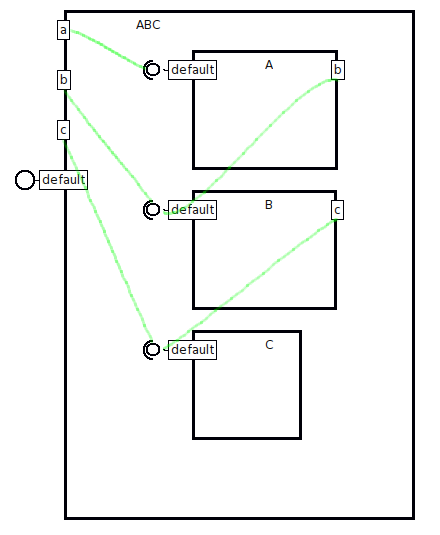
\includegraphics[scale=0.55, keepaspectratio=true]{abc}
\caption{Schéma du programme extrait de \texttt{Compobrowser2}}
\label{abc}
\end{figure}

\begin{lstlisting}[language=Java, frame=single, caption=Workspace]
| prog |
prog := ABC.new();
prog.bar(); "Affiche Hello dans le Transcript"
prog.foo(); "Supprime la connexion entre B et C"
prog.bar(); "Provoque une erreur" 
\end{lstlisting}

L'invocation du service \texttt{bar} ligne 5 lancera l'exception suivante car foo aura coupé la connexion.


\begin{lstlisting}[language=Java, frame=single, caption=Erreur lors de l'exécution du 2e bar(),label=exceptionnotconnected]
Port is not connected
\end{lstlisting}


\begin{lstlisting}[language=Compo, frame=single, caption=Exemple d'une déconnexion à distance]
Descriptor ABC extends Component
{
	provides {
		default: { foo(); bar(); };
	}
	
	internally requires {
		a : A;
		b : B;
		c : C;
	}
	
	architecture {
		connect a@self to default@(A.new());
		connect b@self to default@(B.new());
		connect c@self to default@(C.new());
		
		connect b@a to default@b;
		connect c@b to default@c;
	
	}
	
	service foo (){
		a.fooA();
	}
	
	service bar() {
		a.barA();
	}
}
\end{lstlisting}



\clearpage

\begin{lstlisting}[language=Compo, frame=single, caption=Programme A]
Descriptor A extends Component
{
	provides {
		default: {
			fooA();	barA();
		 };
	}
	
	requires {
		b : B;
	}
	
	service fooA() {
		disconnect c@(b@self) from default@(c@(b@self));
	}
	
	service barA() {
		b.barB();
	}
}
\end{lstlisting}


\begin{lstlisting}[language=Compo, frame=single, caption=Programme B]
Descriptor B extends Component
{
	provides {
		default: { barB(); };
	}
	
	requires {
		c : C;
	}
	
	service barB() {
		c.barC();
	}
}
\end{lstlisting}

\begin{lstlisting}[language=Compo, frame=single, caption=Programme C]
Descriptor C extends Component
{
	provides {
		default: { barC(); };
	}
	
	service barC(){
		<!	"Primitive SmallTalk"
		    Transcript crShow: 'Hello'.	 > 
	}
}
\end{lstlisting}




\chapter{Comparaison entre les deux modes de retour en COMPO}
\label{annexeretourcomparaison}

Le but de cette exemple est de montrer la différence entre les deux modes de retours.

Pour cela, on utilise un compteur classique. Un second composant qui est \texttt{suiveur} possède un port \texttt{compteurVal}. Nous allons montrer que l'on peut synchroniser les deux compteurs pour que lorsque l'on incrémente le compteur, le port interne \texttt{compteurVal} du suiveur se met à jour automatiquement.

\begin{figure}[H]
\centering
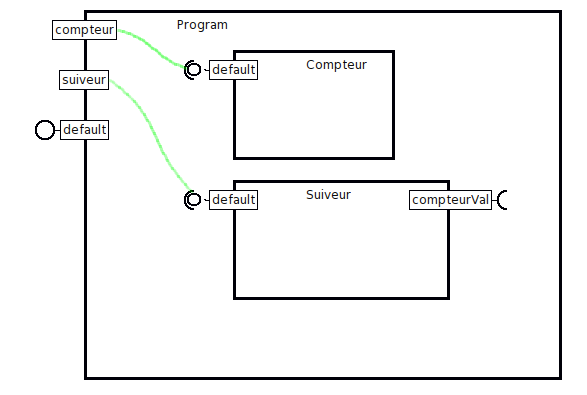
\includegraphics[scale=0.7, keepaspectratio=true]{CompteurSuiveur}
\caption{Schéma du programme extrait de \texttt{Compobrowser2}}
\label{compteursuiveur}
\end{figure}

\clearpage

\begin{lstlisting}[language=Compo, frame=single, caption=Workspace (Retour classique)]
|prog|
prog := Program.new();
prog.init1();

prog.printCompteurs();
prog.inrementer();
prog.printCompteurs();
\end{lstlisting}


\begin{lstlisting}[language=Compo, frame=single, caption=Output (Retour classique)]
compteur : 1
suiveur : 1
Increntation du compteur
compteur : 2
suiveur : 1
\end{lstlisting}

On remarque que lorsque l'on incrémente le compteur, le suiveur n'est pas modifié. En effet, le suiveur s'est connecté directement sur la valeur que possédait le compteur c'est à dire 1. Lorsque l'on incrémente le compteur est modifié. Cependant le suiveur reste connecté à la valeur que on lui avait donnée, autrement dit 1.

\begin{lstlisting}[language=Compo, frame=single, caption=Output (Retour par requis)]
|prog|
prog := Program.new();
prog.init2();

prog.printCompteurs();
prog.inrementer();
prog.printCompteurs();
\end{lstlisting}

\begin{lstlisting}[language=Compo, frame=single, caption=Output (Retour par requis)]
compteur : 1
suiveur : 1
Incrementation du compteur
compteur : 2
suiveur : 2
\end{lstlisting}

Dans cet exemple, le suiveur est bien modifié car on a connecté la valeur du suiveur directement au port qui contient la valeur du compteur et pas à la valeur comme précédemment.


\clearpage

\begin{lstlisting}[language=Compo, frame=single, caption=Le programme]
Descriptor Program extends Component
{
	provides {
		default: {init1(); init2(); incrementer();};
	}
	internally requires {
		compteur : {incrementer();getCompteurVal();getCompteurValReq();printValue();};
		suiveur: {getCompteurVal(); setCompteurVal(cpt);printValue();};
	}
	architecture {
	    compteur >>> default@(Compteur.new());
	    suiveur >>> default@(Suiveur.new());
	}
	operation init1() {
    	suiveur.setCompteurVal(compteur.getCompteurVal());
	}
	operation init2() {
        suiveur.setCompteurVal(compteur.getCompteurValReq());
	}
	operation printCompteurs() {
        compteur.printValue();
        suiveur.printValue();
	}
	operation incrementer(){
        Transcript.crShow('Incrementation du compteur');
        compteur.incrementer();
	}
}
\end{lstlisting}

\begin{lstlisting}[language=Compo, frame=single, caption=Programme Suiveur]
Descriptor Suiveur extends Component
{
	provides {
		default: {getCompteurVal(); setCompteurVal(cptVal);};
	}
	
	requires {
		compteurVal: SmallInteger;
	}
	
	operation getCompteurVal() {
		return compteurVal;
	}
	operation setCompteurVal(cptVal) {
		compteurVal >>> cptVal;
	}
	operation printValue() {
	    Transcript.crShow(compteurVal.asString());
	}
}
\end{lstlisting}

\begin{lstlisting}[language=Compo, frame=single, caption=Programme Compteur]
Descriptor Compteur extends Component
{
	provides {
		default: {incrementer(); getCompteurVal(); getCompteurValReq(); printValue();};
	}
	
	internally requires {
		compteurVal: SmallInteger;
	}
	
	architecture {
	    compteurVal >>> 1;
	}
	
	operation getCompteurVal() {
	    "retourne la valeur connectee"
		return compteurVal;
	}
	
	operation getCompteurValReq() {
	    "retourne le port directement"
		return !compteurVal;
	}
	
	operation incrementer() {
	    | t |
	    t := compteurVal.asString().asInteger() + 1;
	    compteurVal >>> t;
	}
	
	operation printValue() {
	    Transcript.crShow(compteurVal.asString());
	}
}
\end{lstlisting}


\chapter{Comparaison entre les deux modes de passages en COMPO}
\label{passagereqprovider}

Prenons un composant \texttt{A} et un composant \texttt{B}. Tous deux possédent un port \texttt{value}. Le composant \texttt{A} va passer au composant \texttt{B} son port \texttt{value}.

\begin{figure}[H]
\centering
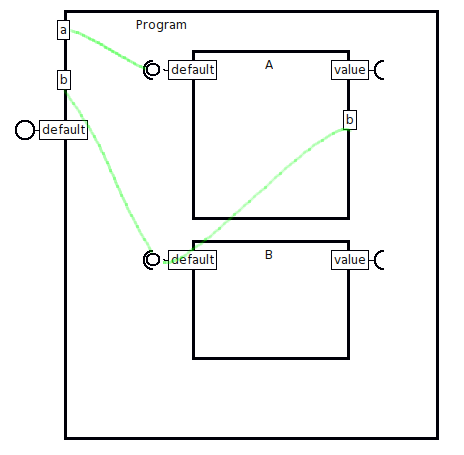
\includegraphics[scale=0.7, keepaspectratio=true]{passagereqprov}
\caption{Schéma du programme extrait de \texttt{Compobrowser2}}
\label{passagereqprov}
\end{figure}



\newpage

\begin{lstlisting}[language=Compo, frame=single, caption=Workspace (Passage par Fournis)]
|prog|
prog := Program.new();
prog.initProv();

prog.printValue();
prog.changeValA();
prog.printValue();
\end{lstlisting}


\begin{lstlisting}[language=Compo, frame=single, caption=Output]
A : 1
B : 1

A : 2
B : 1
\end{lstlisting}

On remarquera que B n'a pas été modifié quand on a modifié ce qui était connecté au port \texttt{value} du composant \texttt{A} avec le mode de passage par défaut.

\begin{lstlisting}[language=Compo, frame=single, caption=Workspace (Passage par Requis)]
|prog|
prog := Program.new();
prog.initReq();

prog.printValue();
prog.changeValA();
prog.printValue();
\end{lstlisting}


\begin{lstlisting}[language=Compo, frame=single, caption=Output]
A : 1
B : 1

A : 2
B : 2
\end{lstlisting}

Avec le mode de passage par requis, cette fois le composant \texttt{B} a bien été modifié en même temps que \texttt{A}

\newpage


\begin{lstlisting}[language=Compo, frame=single, caption=Composant A]
Descriptor A extends Component
{
	provides {
		default : { initProv(); initReq(); print(); setValue(val); };
	}
	
	requires {
		value : SmallInteger;
		b : B;
	}

	operation setValue(val){
	    value >>> val;												
	}
	
	operation initProv() {
		b.setValue(value);	
	}																								
	operation initReq() {
		b.setValue(!value);
	}
	
	operation print() {
		Transcript.crShow(value);
	}
}
\end{lstlisting}

\begin{lstlisting}[language=Compo, frame=single, caption=Composant B]
Descriptor B extends Component
{
	provides {
		default : { setValue(v); print();};
	} 
	
	requires {
		value: SmallInteger;
	}
	
	operation setValue(v) {
		value >>> v;
	}
	
	operation print() {
		Transcript.crShow('' value.asString());
	}
}
\end{lstlisting}

\newpage

\begin{lstlisting}[language=Compo, frame=single, caption=Programme]
Descriptor Program extends Component
{
	provides {
		default : {printValues(); changeValA(); initProv(); initReq(); };
	} 
	
	internally requires {
		a: A;
		b: B;
	}
	
	architecture {
		a >>> default@(A.new());
		b >>> default@(B.new());
		b@a >>> default@b;
		value@a >>> 1;
	}
	
	operation printValues(){
	   a.print();
	   b.print();
	}
	
	operation changeValA(){
	    a.setVal(2);
	}
	
	operation initProv(){
	    a.initProv();
	}
	
	operation initReq(){
	    a.initReq();
	}
	
}
\end{lstlisting}





\chapter{Création d'une règle pour le \textit{parser}}

COMPO utilise le \textit{framework} \texttt{PetitParser} pour l'analyse syntaxique. Il permet la création d'un \textit{AST} grâce à des règles de constructions. Nous allons étudier comment COMPO utilise \texttt{PetitParser}.

\section*{Les différents \textit{packages}}

\subsubsection{Compo parser core}
Ce \textit{package} contient principalement deux classes à savoir :

\begin{itemize}
\item \texttt{PPCompoGrammar} : contient les règles syntaxique
\item \texttt{PPCompoParser} : création des "nodes"
\end{itemize}
	
\subsubsection{Compo parser node}
Ce package contient une série de nodes, les nodes ont leurs propres attributs mais surtout implémentent une méthode nommée \texttt{visitNode}.
Par la suite, un autre élément va parcourir ces nodes grâce à l'implémentation du design pattern "visiteur" afin de générer du code.

\subsubsection{Compo parser visitor}
Ce package est l'élément de l'implémentation qui va s'occuper de parcourir les nodes, il contient une classe très importante nommé
CompoToSmalltalk, cette classe a pour but de généré du code Smalltalk.

\section*{Fonctionnement du parseur}
Le point d'entrée du \textit{parseur} est à la méthode \texttt{start} de \texttt{PPCompoGrammar}. Elle est appelée lorsque l'on fait \textit{accept} dans \texttt{CompoBrowser}.

\section*{Création d'une règle}
Il faut d'abord créer un attribut de classe du nom de la règle qu'on va créer, ensuite il suffit de faire une méthode du même nom, 
et renvoyer un token que PetitParser va comprendre. Ce token ressemble à une expression régulière, voici quelques exemple de règles extrait de \citep{rulesParseur}
\begin{itemize}
\item  Création d'un literal
    \begin{itemize}
    \item (<nom du literal> asParser) 
    \item Ex :  ('connect' asParser);
    \end{itemize}
\item  Pour la détection de nombre, chaine de caractere, ... des symboles ont été crée : $\#letter$, $\#word$, ...;

\item Détection d'un \textit{token} [0..n]
    \begin{itemize}
    \item <token> star
    \item Ex : (('connect' asParser) star); 
    \end{itemize}

\item Détection d'un \textit{token} [1..n]
    \begin{itemize}
    \item <token> plus;
    \item  Ex : (('connect' asParser) plus); 
    \end{itemize}

\item Detection de la suite token1 puis token2 : <token1>, <token2>;
\item  Detection token2 si token1 echoue : (<token1> / <token2>);
\end{itemize}

Ensuite, il suffit de rajouter une méthode du même nom dans PPCompoParser et de la définir ainsi :


\begin{lstlisting}[language=Compo, frame=single, caption=Création d'une régle]
<ma_nouvelle_regle>
	^ super <ma_nouvelle_regle>
\end{lstlisting}
	
PPCompoParser herite de PPCompoGrammar, ainsi la règle est implémentée et prête à l'utilisation.

\section*{Création d'un node}
Là, il n'y a pas grande chose à faire, il suffit de faire une sous classe de \texttt{PPCompoNode}, et d'ajouter à cette classe la méthode \texttt{visitNode}, 
qui va appeler une méthode qu'on définit dans \texttt{CompoToSmalltalk} avec comme argument, lui même.

\section*{Génération de code}
Maintenant, on écrit la méthode dans \texttt{CompoToSmalltalk}. Cette méthode prend en argument le node.
Afin de générer du code, on utilise l'objet CodeStream, qui a une méthode NextPutAll qui prend le code en argument et qui génère le code.

\section*{Problème des littéraux (rock bottom)}
COMPO est fait de façon à ce que lors que l'on écrit

\begin{lstlisting}[language=Compo, frame=single, caption=]
connect <lport>@<lcomp> to <rport>@<rcomp>
\end{lstlisting}

\texttt{lcomp} et \texttt{rcomp} sont des
chaines de caractères (du moins dans la clause architecture). La déduction des chaines de caractère est faite lors de la création des connexions dans \texttt{ComponentBuilder}. Ainsi, pour un littéral, en plus d'ajouter la règle syntaxique, il faut
corriger le comportement de ce \texttt{ComponentBuilder} afin qu'il detecte les litéraux.


\end{appendices}
\glsaddall

\end{document}
